% last updated: 2026-10-11 commit=104de05
% (the line above is read and rewritten by /tidy: the date and the git commit the content of this report describes)
% Research log: what has been implemented in research/, at the level of ideas (no code).
% Build:  python pipeline/tools/build_research_log.py   (pdflatex twice; writes docs/research_log.pdf only)
% Figure paths are relative to docs/. Only `key` outputs of the research modules are included (they are committed,
% so the report builds from a clean clone); the diagrams are drawn here (TikZ).
\documentclass[11pt,a4paper]{article}

\usepackage[T1]{fontenc}
\usepackage[utf8]{inputenc}
\usepackage{lmodern}
\usepackage{microtype}
\usepackage[a4paper,margin=2.5cm,headheight=14pt]{geometry}
\usepackage{amsmath,amssymb}
\usepackage{booktabs,tabularx,array}
\usepackage{graphicx}
\usepackage{xcolor}
\usepackage{enumitem}
\usepackage{float}
\usepackage[font={small,sf},labelfont={small,sf}]{caption}
\usepackage{titlesec}
\usepackage{fancyhdr}
\usepackage{tikz}
\usetikzlibrary{arrows.meta,positioning,calc,patterns,decorations.pathreplacing,fit}
\usepackage{pgfplots}
\pgfplotsset{compat=1.16}
\usepackage[colorlinks=true,linkcolor=navy,urlcolor=navy,citecolor=navy]{hyperref}

\definecolor{navy}{RGB}{26,54,104}
\hypersetup{pdftitle={From measured attenuation to a wet-antenna law: research log}, pdfauthor={Yonatan Haber and Yehonatan Tsitseluk}}
\titleformat{\section}{\Large\sffamily\bfseries}{\thesection}{0.8em}{}
\titleformat{\subsection}{\large\sffamily\bfseries}{\thesubsection}{0.8em}{}
\titleformat{\subsubsection}{\normalsize\sffamily\bfseries}{\thesubsubsection}{0.8em}{}
\pagestyle{fancy}
\fancyhf{}
\fancyhead[L]{\small\sffamily Research log: baseline and wet-antenna attenuation}
\fancyfoot[C]{\small\sffamily\thepage}
\renewcommand{\headrulewidth}{0.6pt}
\setlength{\parskip}{0.5em}
\setlength{\parindent}{0pt}
\setlist{itemsep=0.15em,topsep=0.3em}
\renewcommand{\arraystretch}{1.15}

\newcommand{\Arain}{A_{\mathrm{rain}}}
\newcommand{\Rbar}{\bar{R}}
\newcommand{\dB}{\,\mathrm{dB}}
\newcommand{\code}[1]{\texttt{#1}}
\newcommand{\tzero}{t_{0}}
\newcommand{\ttrace}{t_{\mathrm{trace}}}
\newcommand{\Astart}{A_{\mathrm{start}}}
\newcolumntype{Y}{>{\raggedright\arraybackslash}X}

% a framed "in short" box
\newcommand{\inshort}[1]{\par\smallskip\noindent\fbox{\parbox{\dimexpr\linewidth-2\fboxsep-2\fboxrule-6pt}{\sffamily\small\textbf{In short.} #1}}\par\smallskip}

% diagram styles: status is shown by the border and by a text label, never by colour alone
\tikzset{
  box/.style={draw, rounded corners=2pt, align=center, font=\sffamily\small, inner sep=5pt, minimum height=9mm},
  done/.style={box, line width=1.2pt, fill=black!12},
  doing/.style={box, line width=1.2pt, dashed, fill=black!4},
  todo/.style={box, densely dotted, line width=0.9pt},
  arr/.style={-{Stealth[length=2.2mm]}, line width=0.7pt},
  lab/.style={font=\sffamily\scriptsize, align=center},
}

\begin{document}
\thispagestyle{plain}

\begin{center}
{\LARGE\sffamily\bfseries From measured attenuation to a wet-antenna law\par}
\vspace{0.6em}
{\large\sffamily Research log: what has been implemented, where we stand, and what comes next\par}
\vspace{1.4em}
{\large Yonatan Haber and Yehonatan Tsitseluk\par}
\vspace{0.3em}
CellEnMon lab, final-year electrical engineering project\par
Data-driven discovery of rain-induced and wet-antenna attenuation laws in commercial microwave links\par
\vspace{0.6em}
11 October 2026
\end{center}

\vspace{1em}
\begin{center}{\sffamily\bfseries Abstract}\end{center}

This report describes the research part of the project at the level of ideas: what each step does, why it is done
that way, and what it found. It contains no code. Two things are finished and frozen. First, a \emph{baseline} for
every link and rain event, which turns the raw signal levels into the attenuation $A(t)$; it is unbiased, accurate to
about $\pm 0.2\dB$ per event, and it does not absorb the drying of the antenna after rain. Second, a fixed set of
\emph{drying tails}: 429 stretches of $A(t)$ after the rain has stopped on a link, in which the remaining attenuation
is mostly wet-antenna attenuation (WAA). One thing is in progress: before any drying law is fitted to the real tails,
the fitting method is tested on simulated tails whose true law is known. A fit of one tail at a time cannot tell the
candidate laws apart; a fit of all tails together can, on simulated data. A stress test of that fit passed for three
of the four laws tested and showed that two of the nonlinear laws cannot be told apart from each other. The second
tool, SINDy, has not been tested yet. No law has been fitted to real tails yet. Still to come are the drying law itself (fitting and weak-form SINDy), the
wetting law from very short links, the verification on unseen events, and then the two later stages of the project:
the path law $f(L,\Rbar,Z)$ and the rain estimate.

\vspace{0.5em}
\tableofcontents
\newpage

% =====================================================================================================================
\section{Scope and status at a glance}

\subsection{What this report covers}

The report covers the research folder of the repository as it stood on 11 October 2026: the baseline module and the
WAA module. The data layer below it (the pipeline that turns the raw OpenMRG files into a verified data set) has its
own technical report and is summarised here in one page (Section~\ref{sec:data}). Every number in this report is
taken from the documents the two modules keep: their method descriptions, their decision logs and their step reports
(Appendix~\ref{app:where}). Unless stated otherwise, the numbers are for the \emph{training} events and
\emph{training} links only; the validation set is built by the same rules but has not been looked at, and the test set
has not been touched.

References in square brackets are those of the project proposal and are listed at the end.

\subsection{Status}

Figure~\ref{fig:roadmap} shows the whole project and Table~\ref{tab:status} the steps inside it.

\begin{figure}[H]
\centering
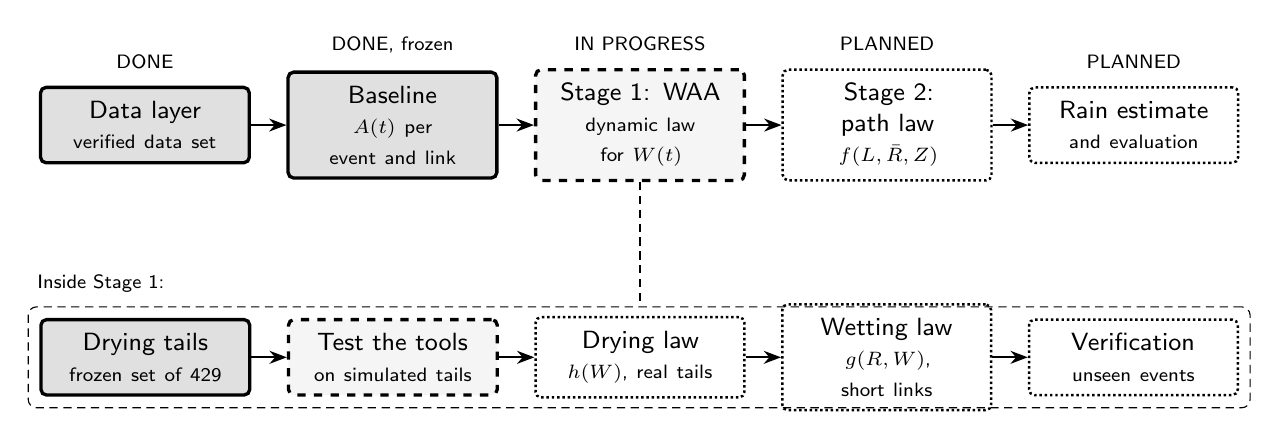
\begin{tikzpicture}[node distance=5mm and 4.5mm]
\node[doing, text width=23mm] (waa) {Stage 1: WAA\\{\scriptsize dynamic law for $W(t)$}};
\node[done, text width=23mm, left=of waa] (base) {Baseline\\{\scriptsize $A(t)$ per event and link}};
\node[done, text width=23mm, left=of base] (data) {Data layer\\{\scriptsize verified data set}};
\node[todo, text width=23mm, right=of waa] (path) {Stage 2: path law\\{\scriptsize $f(L,\Rbar,Z)$}};
\node[todo, text width=23mm, right=of path] (eval) {Rain estimate\\{\scriptsize and evaluation}};
\draw[arr] (data) -- (base);
\draw[arr] (base) -- (waa);
\draw[arr] (waa) -- (path);
\draw[arr] (path) -- (eval);
\node[lab, above=1mm of data] {DONE};
\node[lab, above=1mm of base] {DONE, frozen};
\node[lab, above=1mm of waa] {IN PROGRESS};
\node[lab, above=1mm of path] {PLANNED};
\node[lab, above=1mm of eval] {PLANNED};
% inside stage 1
\node[todo, text width=23mm, below=17mm of waa] (s3) {Drying law\\{\scriptsize $h(W)$, real tails}};
\node[doing, text width=23mm, left=of s3] (s2) {Test the tools\\{\scriptsize on simulated tails}};
\node[done, text width=23mm, left=of s2] (s1) {Drying tails\\{\scriptsize frozen set of 429}};
\node[todo, text width=23mm, right=of s3] (s4) {Wetting law\\{\scriptsize $g(R,W)$, short links}};
\node[todo, text width=23mm, right=of s4] (s5) {Verification\\{\scriptsize unseen events}};
\draw[arr] (s1) -- (s2); \draw[arr] (s2) -- (s3); \draw[arr] (s3) -- (s4); \draw[arr] (s4) -- (s5);
\node[draw, densely dashed, rounded corners=3pt, inner sep=4pt, fit=(s1)(s5)] (grp) {};
\node[lab, anchor=south west] at ($(grp.north west)+(0,0.5mm)$) {Inside Stage 1:};
\draw[densely dashed] (waa.south) -- (waa.south |- grp.north);
\end{tikzpicture}
\caption{The project, and the inside of Stage~1. Thick solid border with grey fill: done. Thick dashed border: in
progress. Dotted border: planned.}
\label{fig:roadmap}
\end{figure}

\begin{table}[H]
\centering
\caption{Steps of the research part and their state on 11 October 2026.}
\label{tab:status}
\small
\begin{tabularx}{\linewidth}{@{}l Y l l@{}}
\toprule
\textbf{Step} & \textbf{What it is} & \textbf{State} & \textbf{Section} \\
\midrule
Baseline & Dry-weather level per (event, sub-link); $A(t)$ & done, frozen 7 Oct & \ref{sec:baseline} \\
WAA 0--1 & Inventory; extract every drying tail (20\,355) & done & \ref{sec:tails} \\
WAA 2, 2b, 2c & Selection by fixed rules; frozen tail set v1 (429 train, 123 validation) & done, frozen 8 Oct & \ref{sec:tails} \\
WAA 3a & Simulator of tails, calibrated to the real set & done & \ref{sec:sim} \\
WAA 3b-1 & Fit one tail at a time, on simulated tails & done: not enough & \ref{sec:pertail} \\
WAA 3b-1b & Fit all tails together, on simulated tails & done: works & \ref{sec:pooled} \\
WAA 3b-1c & Stress test of that fit & done: partly passed & \ref{sec:stress} \\
WAA 3b-2, 3c & SINDy on simulated tails; simulator of whole events & not started & \ref{sec:next} \\
WAA 4--6 & Drying law $h(W)$ on real tails; what it depends on & not started & \ref{sec:next} \\
WAA 7 & Wetting law $g(R,W)$ from very short links & not started & \ref{sec:next} \\
WAA 8--9 & Verification; final WAA equation & not started & \ref{sec:next} \\
Stage 2 & Path law $f(L,\Rbar,Z)$ with symbolic regression & not started & \ref{sec:next} \\
Evaluation & Rain estimate, comparison with the literature & not started & \ref{sec:next} \\
\bottomrule
\end{tabularx}
\end{table}

% =====================================================================================================================
\section{The problem in equations}
\label{sec:problem}

\subsection{What a link measures}

A commercial microwave link (CML) sends a signal from one mast to another. The network records the transmitted
signal level (TSL) and the received signal level (RSL). Their difference is the total loss
$\mathrm{TL}(t) = \mathrm{TSL}(t) - \mathrm{RSL}(t)$. Most of it is always there (free-space loss, cables, antennas).
What is always there is called the \emph{baseline}, and the \emph{attenuation} is what is left above it:
\begin{equation}
A(t) \;=\; \mathrm{TSL}(t) - \mathrm{RSL}(t) - \text{baseline} \;=\; \Arain(t) + \delta(t).
\label{eq:A}
\end{equation}
$\Arain$ is the loss caused by rain along the path. $\delta(t)$ collects everything else, mainly wet-antenna
attenuation and whatever error is left in the baseline.

\subsection{Rain along the path}

Every short piece $dx$ of the path attenuates the signal by $a\,R(x,t)^{b}\,dx$, where $R(x,t)$ is the local rain
rate and $a$, $b$ depend on the frequency and polarisation. The link sums all pieces:
\begin{equation}
\Arain(t) \;=\; \int_{0}^{L} a\,R(x,t)^{b}\,dx \;\approx\; a\,\Rbar(t)^{b}\,L ,
\label{eq:powerlaw}
\end{equation}
with $L$ the path length and $\Rbar$ the mean rain rate along the path. The approximation is exact only when the rain
is uniform along the path. The project replaces it by a more general form,
\begin{equation}
\Arain(t) \;=\; a\,\Rbar(t)^{b}\,f(L,\Rbar,Z),
\label{eq:f}
\end{equation}
where $f$ is a correction function to be found from data and $Z$ stands for properties of the path and the link
(non-uniform rain, frequency, polarisation, time resolution). Uniform rain gives $f = L$.

\subsection{Wet-antenna attenuation, and why it comes first}

Water collects on the antenna covers during rain and dries afterwards. This adds an attenuation $W(t)$, the WAA. It
differs from $\Arain$ in two ways: it is local (it happens at the two antennas, so it does not grow with $L$), and it
has memory (it stays after the rain has stopped).

WAA has to be removed before $f$ is learned. Suppose the WAA were a constant $W$. Then
\begin{equation}
A = a\Rbar^{b}L + W
\quad\Longrightarrow\quad
\frac{A}{a\Rbar^{b}} = L + \underbrace{\frac{W}{a\Rbar^{b}}}_{L_{0}} ,
\label{eq:L0}
\end{equation}
so a constant WAA looks exactly like a path that is longer by $L_{0}$. A method that learns $f$ from $A$ would
return $f = L + L_{0}$ and report a length dependence that is not there. This fixes the order of the work
(Figure~\ref{fig:chain}): baseline, then WAA, then $f$.

\begin{figure}[H]
\centering
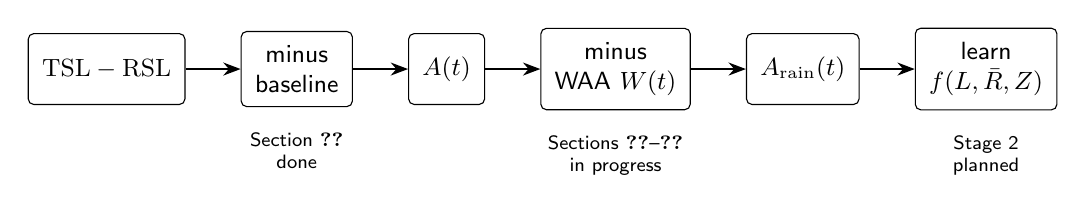
\begin{tikzpicture}[node distance=7mm]
\node[box] (tl) {$\mathrm{TSL}-\mathrm{RSL}$};
\node[box, right=of tl] (b) {minus\\baseline};
\node[box, right=of b] (a) {$A(t)$};
\node[box, right=of a] (w) {minus\\WAA $W(t)$};
\node[box, right=of w] (ar) {$\Arain(t)$};
\node[box, right=of ar] (f) {learn\\$f(L,\Rbar,Z)$};
\draw[arr] (tl)--(b); \draw[arr] (b)--(a); \draw[arr] (a)--(w); \draw[arr] (w)--(ar); \draw[arr] (ar)--(f);
\node[lab, below=2mm of b] {Section~\ref{sec:baseline}\\done};
\node[lab, below=2mm of w] {Sections~\ref{sec:tails}--\ref{sec:tools}\\in progress};
\node[lab, below=2mm of f] {Stage 2\\planned};
\end{tikzpicture}
\caption{The order of the work. An error in an early block is passed on to every later block, which is why each block
is validated and frozen before the next one starts.}
\label{fig:chain}
\end{figure}

\subsection{Three rules that shape every step}

\begin{enumerate}
\item \textbf{No circular selection.} Links or events are never chosen by how well a model fits them. Choosing the
links where the power law works, and then concluding that the power law works, would prove nothing. Every selection
rule in this report is fixed before the result is seen and never looks at the shape of the curve.
\item \textbf{Readable equations.} The aim is an explicit law that can be checked against the physics (a
\emph{gray-box} model), not only a good prediction. A neural network [11] is used later only as a reference for
performance.
\item \textbf{Rain is defined by the references, never by the link.} Whether it rains on a link is decided from the
weather radar along the path and from the rain gauges. The link's own signal is never used for that, because the
signal is the thing being explained.
\end{enumerate}

% =====================================================================================================================
\section{What the data layer provides}
\label{sec:data}

The research uses the OpenMRG data set [13]: three summer months (June to August 2015) of 364 two-way links (728
sub-links, one per direction) around Gothenburg, with ten city rain gauges, one national gauge with weather data, and
a weather-radar composite. The points that matter for the research are these.

\begin{itemize}
\item \textbf{Resolution.} The links are sampled every 10 s. RSL is recorded in steps of $0.3\dB$ and TSL in steps of
$1\dB$. This \emph{quantization} is the size of the effects studied here, so it appears in almost every section.
\item \textbf{Rain reference.} The radar gives the rain rate every 5 minutes on a 2 km grid; the data layer averages
it along each link path to get $\Rbar$. The radar is preferred over a single gauge because it sees the whole path.
\item \textbf{Rain events.} 89 rain events and 62 long dry periods are defined from the radar and the gauges only.
\item \textbf{Reference state of each link.} Every 5 minutes each link is labelled \emph{wet} (radar on the path or a
gauge within 1 km shows at least $0.1$ mm/h), \emph{dry} (no rain at all on the path in that bin and for 30 minutes
on either side), or \emph{unknown} (anything in between, or radar missing). Unknown never counts as dry.
\item \textbf{Split.} Events are divided into training, validation and test sets (60 / 20 / 20 \%), and links into
training and test (80 / 20 \%). The split is frozen. The training set has 283 links (566 sub-links).
\end{itemize}

% =====================================================================================================================
\section{Step 1: the baseline and $A(t)$ (done, frozen)}
\label{sec:baseline}

\subsection{The idea and the main risk}

The baseline is the total loss a sub-link would show if it were not raining. It cannot be measured during rain, so it
has to be estimated from dry time. The main risk is specific to this project. After the rain stops, the antenna is
still wet and the signal returns slowly. If the baseline is estimated from that period, or is allowed to move during
the event, it follows the slow return and the wet-antenna attenuation disappears into the baseline, which is exactly
the signal Stage~1 needs. The baseline must therefore be blind to everything that happens after the event starts.

\subsection{The method}

For each pair of a rain event $e$ and a sub-link $s$, the baseline is one number: the median of the total loss over
the usable dry time in the 24 hours before the event starts,
\begin{equation}
\begin{aligned}
B_{e,s} &= \operatorname*{median}\bigl\{\, \mathrm{TL}_{s}(t) \;:\; t \in [\,t_{\mathrm{start}}(e) - 24\,\mathrm{h},\; t_{\mathrm{start}}(e)\,),\ t \text{ usable} \,\bigr\}, \\
A_{s}(t) &= \mathrm{TL}_{s}(t) - B_{e,s} .
\end{aligned}
\label{eq:baseline}
\end{equation}
A 5-minute slot is \emph{usable} if the link's reference state is dry and at least one hour has passed since the link
was last wet (so that the drying of an earlier shower is kept out). If the 24-hour window holds less than one hour of
usable time, a 48-hour window is used; if that fails too, the pair gets no baseline rather than a guess. This happens
for 2.9\,\% of the pairs, almost all of them in the first events of the season, which have no history before them.
Figure~\ref{fig:window} shows the construction.

\begin{figure}[H]
\centering
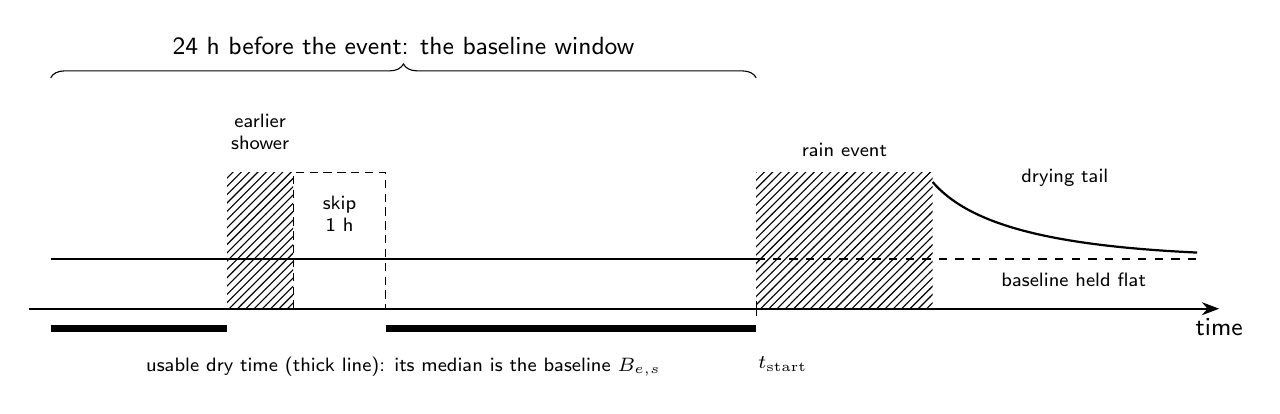
\begin{tikzpicture}[x=0.56cm,y=1.15cm]
\draw[arr] (-0.5,0) -- (26.5,0) node[below, font=\sffamily\small] {time};
\draw[decorate, decoration={brace, amplitude=5pt}] (0,2.55) -- (16,2.55) node[midway, above=5pt, font=\sffamily\small] {24 h before the event: the baseline window};
% earlier shower and the skip after it
\fill[pattern=north east lines] (4,0) rectangle (5.5,1.5);
\node[lab] at (4.75,1.95) {earlier\\shower};
\draw[densely dashed] (5.5,0) rectangle (7.6,1.5);
\node[lab] at (6.55,1.05) {skip\\1 h};
% usable time
\draw[line width=2.4pt] (0,-0.22) -- (4,-0.22);
\draw[line width=2.4pt] (7.6,-0.22) -- (16,-0.22);
\node[lab, anchor=north] at (8,-0.42) {usable dry time (thick line): its median is the baseline $B_{e,s}$};
% event
\fill[pattern=north east lines] (16,0) rectangle (20,1.5);
\node[lab] at (18,1.75) {rain event};
\node[lab] at (23,1.45) {drying tail};
% baseline level
\draw[line width=1pt] (0,0.55) -- (16,0.55);
\draw[line width=1pt, dashed] (16,0.55) -- (26,0.55);
\node[lab, anchor=north] at (23.2,0.5) {baseline held flat};
\draw[line width=0.8pt] (20,1.4) .. controls (20.8,0.95) and (22.5,0.7) .. (26,0.62);
\draw (16,0.08) -- (16,-0.08);
\node[lab, anchor=north] at (16.6,-0.42) {$t_{\mathrm{start}}$};
\end{tikzpicture}
\caption{The baseline of one event on one sub-link. Only dry time before the event is used, so the baseline cannot
follow the drying tail. Hatched: rain according to the references.}
\label{fig:window}
\end{figure}

A first version of the method (v1) used the mean over 6 hours before the event, and in some cases a sloping line
from the level before the event to the level after it. The frozen version (v2) differs in three choices, each one
decided by the validation below: a longer window (24 h), the median instead of the mean, and a flat baseline only.
The sloping line was dropped because the cases where it applied did not look like drying; they looked like changes of
level that have nothing to do with the rain.

\subsection{How a baseline is validated when the truth is unknown}

There is no ``true'' baseline to compare with during rain. The idea of the validation is to create cases where the
truth \emph{is} known. In certified dry weather the attenuation is zero by definition. So we place \emph{fake events}
in dry periods: we pretend that an event of duration $D$ starts at a random dry moment, compute the baseline exactly as
for a real event, and measure what the method reports during the fake event. Anything other than zero is baseline
error. The error of one fake event is its \emph{offset},
\begin{equation}
\text{offset} \;=\; \frac{1}{D}\int_{\text{fake event}} \bigl(\mathrm{TL}(t) - B\bigr)\,dt , \qquad \text{truth} = 0 .
\end{equation}
This was done for 513 good training sub-links, six durations from 1 to 40 hours and 20 fake events each: 61\,560 fake
events. Table~\ref{tab:offset} gives the result.

\begin{table}[H]
\centering
\caption{Baseline error on fake events in dry weather (truth: zero). ``90\,\% within'' is the 90th percentile of
$|\text{offset}|$. The summer median is the simplest possible baseline (one number per sub-link for the whole
season).}
\label{tab:offset}
\small
\begin{tabular}{@{}lcccccc@{}}
\toprule
 & \multicolumn{6}{c}{Duration $D$ of the fake event} \\
\cmidrule(l){2-7}
90\,\% of offsets within (dB) & 1 h & 3 h & 6 h & 12 h & 24 h & 40 h \\
\midrule
Summer median & 0.43 & & 0.40 & & 0.34 & \\
v1: 6 h mean before the event & 0.29 & 0.31 & 0.34 & 0.36 & 0.30 & 0.38 \\
\textbf{v2: 24 h median before the event} & 0.33 & 0.32 & 0.31 & 0.28 & 0.28 & 0.29 \\
\midrule
v2: median offset & $0.00$ & $0.00$ & $0.00$ & $0.00$ & $+0.02$ & $+0.05$ \\
\bottomrule
\end{tabular}
\end{table}

What the table says:
\begin{itemize}
\item The baseline is \textbf{unbiased}: the median offset is zero.
\item Its \textbf{spread is about $\pm 0.2\dB$} (10th to 90th percentile), and 90\,\% of the errors are below about
$0.3\dB$. That is one RSL quantization step: the baseline is about as accurate as the instrument allows.
\item The short window (v1) is slightly better for events of 1 to 3 hours, the long window (v2) is better from 6
hours on. Real significant events last several hours, so v2 was chosen.
\end{itemize}

\subsection{Does the baseline absorb the drying?}

This is the check the proposal asks for. After each real event we measure how far the signal is above the baseline
$k$ hours after the link's last wet moment, and compare with the same quantity after fake events (the control, where
nothing dries). If the baseline had swallowed the drying, the real and the control curves would be equal at all $k$.
Figure~\ref{fig:delta} shows a small excess after real rain ($+0.04\dB$ above the control one hour after the rain)
that shrinks to zero by 12 hours. The drying signal stays in $A(t)$, as intended. The excess is small in the median
because most (event, sub-link) pairs have little rain; the strong cases are selected in Section~\ref{sec:tails}.

\begin{figure}[H]
\centering
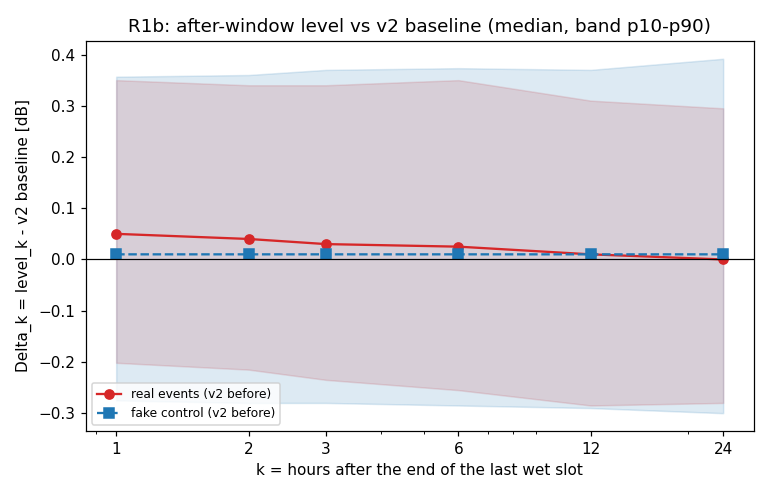
\includegraphics[width=0.62\linewidth]{../research/baseline_estm/outputs/figures/r1b_c2_delta.png}
\caption{Level after the rain minus the baseline, against the time since the link's last wet moment. Circles, solid
line: real events. Squares, dashed line: control (fake events in dry weather). Bands: 10th to 90th percentile.}
\label{fig:delta}
\end{figure}

\subsection{What disturbs the signal in dry weather}

The validation also showed what the baseline cannot remove, because it happens with no rain at all:
\begin{itemize}
\item \textbf{A daily cycle.} The dry-weather loss of a sub-link moves over the day, by $0.15\dB$ for the median
sub-link but by more than $0.4\dB$ for 14\,\% of them. Those sub-links have about twice the baseline error.
\item \textbf{Dew.} Jumps of $1\dB$ or more in dry weather happen mostly at night in humid air (a third of them at
relative humidity $\geq 90\,\%$, against 5\,\% of all dry time), usually in both directions of a link and on
neighbouring links at once. This is most likely dew on the antennas: wet-antenna attenuation without rain. An hour is
marked ``at dew risk'' when the humidity is at least 90\,\% or the air is within $2\,^{\circ}$C of its dew point.
\end{itemize}
These are not corrected. Instead each (event, sub-link) pair carries \emph{flags} (baseline far from the usual dry
level, large daily cycle, dew risk, degraded link), and the pairs with a serious flag are left out of the main WAA
analysis. One tested idea was rejected by a rule fixed before the run: leaving the dew-risk hours out of the baseline
window did not improve the error, so it was not adopted.

\subsection{What the baseline hands to the next step}

\begin{itemize}
\item One baseline per (event, sub-link), for training and validation events on training links, with its flags.
$A(t)$ follows from Eq.~\eqref{eq:baseline}.
\item One number per sub-link, $\sigma_{\mathrm{off}}$: the spread of its baseline error on fake events. It says how
far $A(t)$ of that sub-link may sit from zero for no physical reason, and it is used later as prior knowledge when
laws are fitted (Section~\ref{sec:pooled}).
\end{itemize}

\inshort{The baseline is the median dry level of the 24 hours before each event, held flat. It is unbiased, accurate
to about one quantization step, and blind to the drying after the rain. Frozen on 7 October 2026.}

% =====================================================================================================================
\section{Stage 1, part 1: the drying tails (done, frozen)}
\label{sec:tails}

\subsection{The idea}

During rain, $A(t)$ is the sum of two unknowns, $\Arain(t)$ and $W(t)$, and they cannot be separated without assuming
a model for one of them. After the rain has stopped on a link, the path term is zero:
\begin{equation}
R(x,t) = 0 \ \text{on the path}
\ \ \Longrightarrow\ \ \Arain(t) = 0
\ \ \Longrightarrow\ \ A(t) = W(t) + \text{baseline error} + \text{noise} .
\label{eq:tail}
\end{equation}
The stretch of $A(t)$ after the rain is called a \emph{drying tail}. In it we observe the WAA almost directly, with
no assumption about the power law. Figure~\ref{fig:tail} shows the picture. The tails show only how the antenna
\emph{dries}; how it \emph{gets wet} has to be learned later from data during the rain
(Section~\ref{sec:next}).

\begin{figure}[H]
\centering
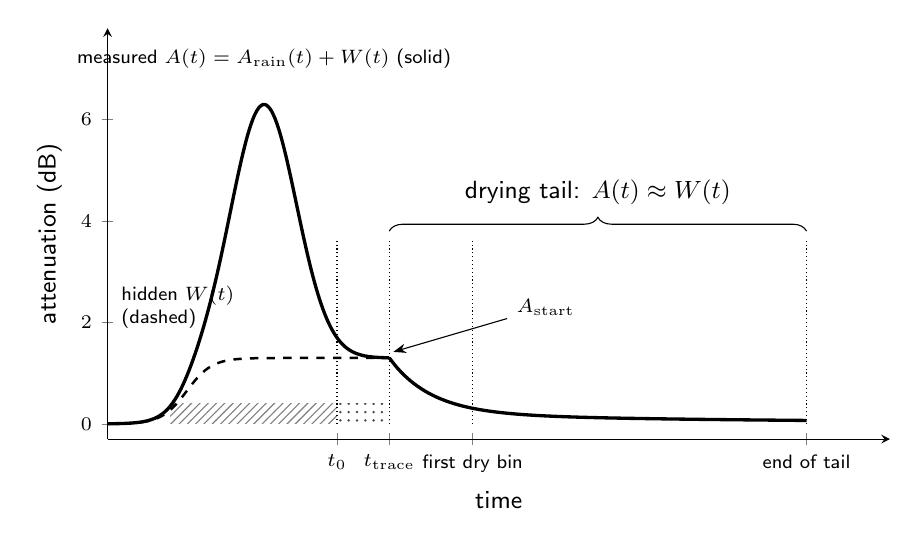
\begin{tikzpicture}
\begin{axis}[width=0.95\linewidth, height=6.8cm, xmin=-135, xmax=240, ymin=-0.3, ymax=7.8,
  axis lines=left, xlabel={time}, ylabel={attenuation (dB)},
  xtick={-25,0,40,200}, xticklabels={$\tzero$,$\ttrace$,first dry bin,end of tail},
  ytick={0,2,4,6}, tick label style={font=\sffamily\scriptsize}, label style={font=\sffamily\small},
  clip=false]
\fill[pattern=north east lines, pattern color=black!50] (axis cs:-105,0) rectangle (axis cs:-25,0.4);
\fill[pattern=dots, pattern color=black!70] (axis cs:-25,0) rectangle (axis cs:0,0.4);
\addplot[domain=-135:0, samples=70, smooth, line width=1.2pt] {5*exp(-((x+60)/22)^2) + 1.3/(1+exp(-(x+97)/6))};
\addplot[domain=0:200, samples=60, smooth, line width=1.2pt] {1.3*(0.85*exp(-x/20)+0.15*exp(-x/190)) + 5*exp(-((x+60)/22)^2)};
\addplot[domain=-135:0, samples=50, smooth, line width=0.9pt, dashed] {1.3/(1+exp(-(x+97)/6))};
\draw[densely dotted] (axis cs:-25,0) -- (axis cs:-25,3.6);
\draw[densely dotted] (axis cs:0,0) -- (axis cs:0,3.6);
\draw[densely dotted] (axis cs:40,0) -- (axis cs:40,3.6);
\draw[densely dotted] (axis cs:200,0) -- (axis cs:200,3.6);
\node[font=\sffamily\scriptsize, align=center] at (axis cs:-60,7.2) {measured $A(t) = \Arain(t) + W(t)$ (solid)};
\node[font=\sffamily\scriptsize, align=left, anchor=west] at (axis cs:-133,2.3) {hidden $W(t)$\\(dashed)};
\draw[decorate, decoration={brace, amplitude=5pt}] (axis cs:0,3.8) -- (axis cs:200,3.8)
  node[midway, above=6pt, font=\sffamily\small] {drying tail: $A(t) \approx W(t)$};
\node[font=\sffamily\scriptsize] (as) at (axis cs:75,2.3) {$\Astart$};
\draw[-{Stealth[length=1.6mm]}, line width=0.4pt] (as) -- (axis cs:2,1.42);
\end{axis}
\end{tikzpicture}
\caption{Sketch of one event on one link (not real data). During the rain the measured attenuation is the sum of the
path term and the hidden WAA. After the last trace of rain, at $\ttrace$, only the WAA is left and it decays as the
antenna dries. Hatched bar: rain on the path according to the references. Dotted bar: only a trace of rain, below the
threshold that makes a bin wet.}
\label{fig:tail}
\end{figure}

\subsection{Extracting every tail, with no selection}

The first step cuts one tail for every (event, sub-link) pair that has a baseline and had rain, using the reference
state of the link only:
\begin{itemize}
\item \textbf{Start} $\tzero$: the end of the link's last wet bin in the event.
\item \textbf{End}: the first of (a) the next wet bin of the link, (b) a gap of 15 minutes or more in the data,
(c) $\tzero + 12$ hours. The end never looks at the value of $A$, so a tail is not forced to reach zero.
\end{itemize}
This gives 20\,355 tails on 566 sub-links from 69 events (15\,370 from training events). Nothing is selected and
nothing is fitted at this point. A first descriptive result already shows that the memory exists: of the tails that
start above $2\dB$, only 25\,\% are back at their dry level after 10 minutes and 79\,\% after 3 hours, while tails
that start below $0.5\dB$ are back within 10 minutes in 94\,\% of the cases.

\subsection{Selection by rules fixed in advance}

Most of the 20\,355 tails are too weak or too disturbed to say anything about drying. The selection uses only rules
that are fixed before the result is seen and that never look at the shape of the decay:
\begin{itemize}
\item \textbf{Exclude} pairs with a flagged baseline, sub-links that are not of good quality, sub-links whose
dry-weather baseline error $\sigma_{\mathrm{off}}$ exceeds $0.3\dB$ (one RSL step), and tails with more than 10\,\% of
missing minutes.
\item \textbf{Shorten} a tail when something other than drying starts: a step in the transmitted power, or a
sustained rise of $A$ (below).
\item \textbf{Main set}: the tail starts at $\Astart \geq 1\dB$ and has at least 60 usable minutes. A larger
\emph{alternative set} uses $\Astart \geq 0.6\dB$ and serves as a sensitivity check.
\item \textbf{Control set}: tails that start below $0.5\dB$. They show what a tail looks like when there is nothing
to dry, and are used to measure the noise (Section~\ref{sec:sim}).
\end{itemize}

\subsection{A lesson: the ``fast drop''}
\label{sec:fastdrop}

The first selection produced 959 main tails, and they showed a striking feature: within the first half hour (the
margin between the last wet bin and the first certified dry bin) the attenuation fell by a median of $1.1\dB$, which
is 83\,\% of its starting value. It was tempting to read this as a fast drying of the antenna. Two checks said
otherwise.
\begin{itemize}
\item The drop did not grow with the link length $L$, which would point to the antenna and not to the path. But the
comparison quantity, the attenuation during the rain, barely grew with $L$ either (rank correlation 0.13), so this
test had little power to decide.
\item Looking at the references more closely showed that in this margin the radar or a gauge often still reported a
\emph{trace} of rain, below the threshold that makes a bin ``wet''. When the start of the tail was moved to the end of
the last trace, 381 of the 959 tails no longer started above $1\dB$.
\end{itemize}
So much of the fast drop was light rain ending, not the antenna drying. The consequence is the stricter start used
from then on, and a clear statement of what is and is not shown: the tails are a clean place to study drying, but the
proof that what dries is the antenna and not residual path rain is left to the test with very short links
(Section~\ref{sec:next}), where the contrast in $L$ is large enough.

\subsection{The frozen tail set v1}

The final rules are:
\begin{itemize}
\item \textbf{Start} $\ttrace$: the end of the last 5-minute bin with any trace of rain (radar above zero on the
path, a gauge within 1 km above zero, or radar missing, which counts as ``unknown, so possibly rain''). $\Astart$ is
the mean of $A$ over the first 5 minutes from $\ttrace$.
\item \textbf{End}: the first of the ends listed above, the first new trace of rain, and the \emph{rise cut}: if $A$
(smoothed over 10 minutes) rises $0.6\dB$ above its lowest value so far and stays there for 10 minutes, the tail
ends just before the rise began. A drying antenna does not get wetter, so a sustained rise means something else has
started.
\end{itemize}
Figure~\ref{fig:funnel} shows how many tails each stage leaves, and Table~\ref{tab:v1} the frozen set.

\begin{figure}[H]
\centering
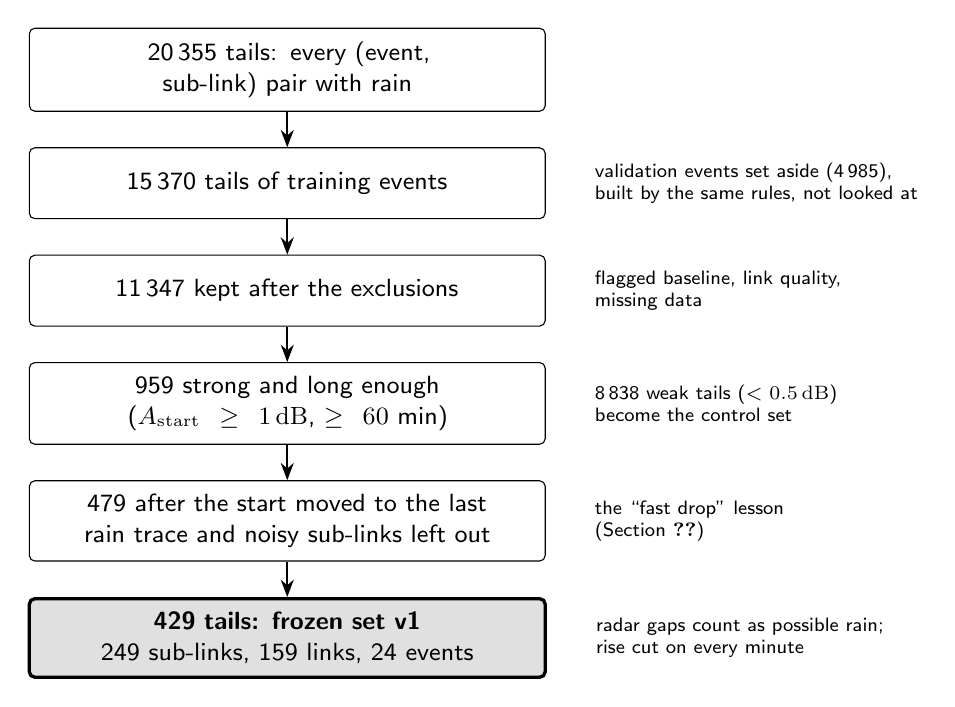
\begin{tikzpicture}[node distance=4.5mm]
\node[box, text width=62mm] (a) {20\,355 tails: every (event, sub-link) pair with rain};
\node[box, text width=62mm, below=of a] (b) {15\,370 tails of training events};
\node[box, text width=62mm, below=of b] (c) {11\,347 kept after the exclusions};
\node[box, text width=62mm, below=of c] (d) {959 strong and long enough\\($\Astart \geq 1\dB$, $\geq 60$ min)};
\node[box, text width=62mm, below=of d] (e) {479 after the start moved to the last rain trace and noisy sub-links left out};
\node[done, text width=62mm, below=of e] (f) {\textbf{429 tails: frozen set v1}\\249 sub-links, 159 links, 24 events};
\foreach \u/\v in {a/b,b/c,c/d,d/e,e/f} \draw[arr] (\u)--(\v);
\node[lab, right=5mm of b, anchor=west, align=left] {validation events set aside (4\,985),\\built by the same rules, not looked at};
\node[lab, right=5mm of c, anchor=west, align=left] {flagged baseline, link quality,\\missing data};
\node[lab, right=5mm of d, anchor=west, align=left] {8\,838 weak tails ($< 0.5\dB$)\\become the control set};
\node[lab, right=5mm of e, anchor=west, align=left] {the ``fast drop'' lesson\\(Section~\ref{sec:fastdrop})};
\node[lab, right=5mm of f, anchor=west, align=left] {radar gaps count as possible rain;\\rise cut on every minute};
\end{tikzpicture}
\caption{From all tails to the frozen set. No stage looks at how the tail decays.}
\label{fig:funnel}
\end{figure}

\begin{table}[H]
\centering
\caption{The frozen tail set v1 (8 October 2026).}
\label{tab:v1}
\small
\begin{tabular}{@{}lrrrr@{}}
\toprule
Set & Tails & Sub-links & Links & Events \\
\midrule
Main, training & 429 & 249 & 159 & 24 \\
Main, validation (not looked at) & 123 & 96 & 76 & 9 \\
Alternative ($\Astart \geq 0.6\dB$), training & 1\,155 & 368 & 212 & 34 \\
Alternative, validation (not looked at) & 458 & 263 & 170 & 12 \\
\bottomrule
\end{tabular}
\end{table}

\subsection{What the tails look like}

Figure~\ref{fig:median} shows the median of the 429 tails. It starts near $1.5\dB$, loses half of its value in about
15 minutes, is at about a quarter after 30 minutes, and then slows down: about 14\,\% is left after one hour and 5\,\%
after three hours. The control tails stay at zero. The shape is \emph{fast at first, slow later}, and the central
question of the next section is what kind of law produces it.

\begin{figure}[H]
\centering
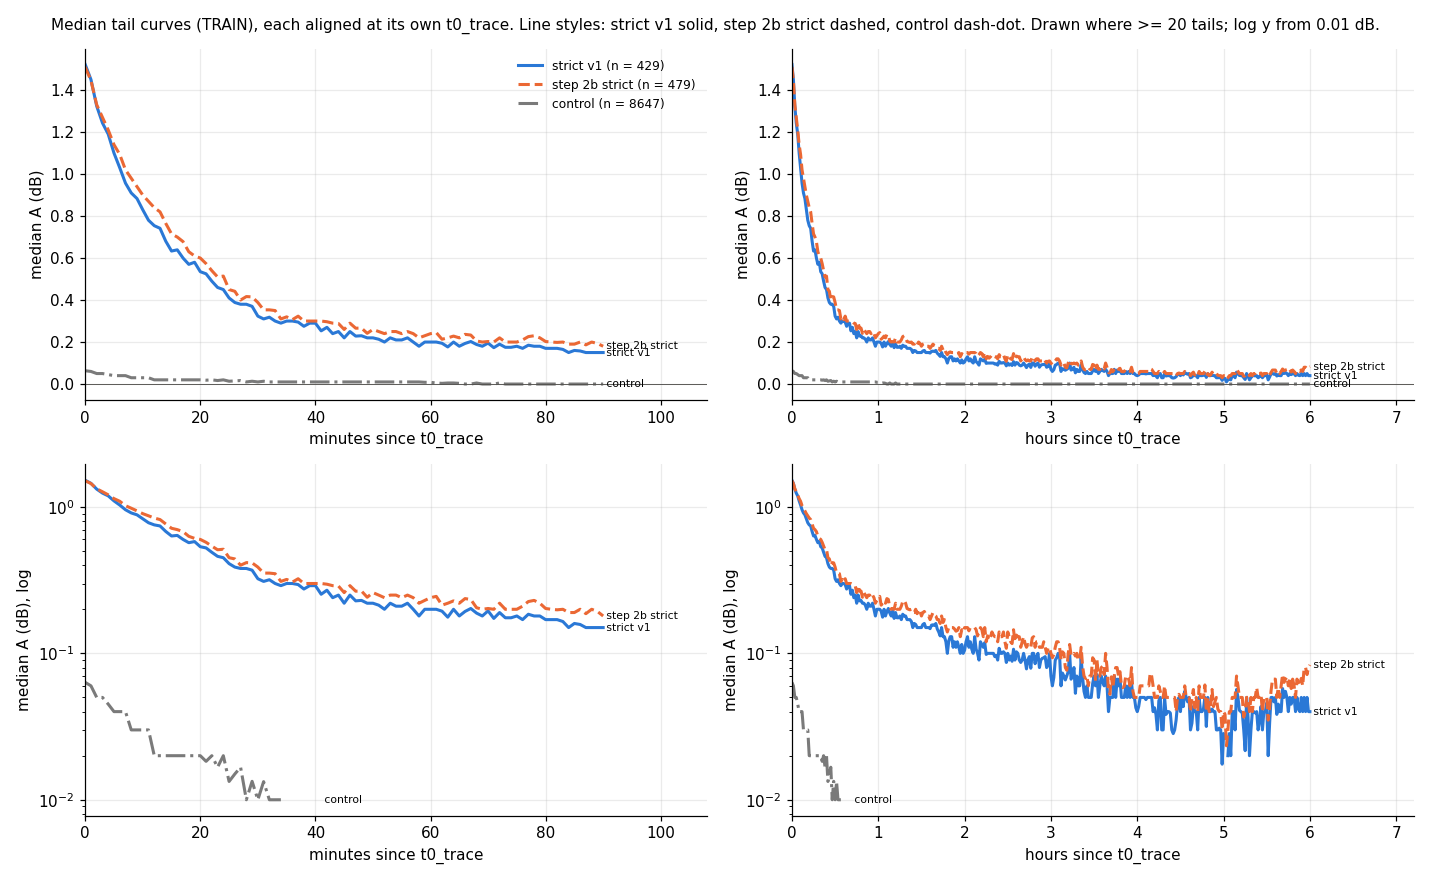
\includegraphics[width=\linewidth]{../research/WAA_estm/outputs/figures/step2c_median_curves.png}
\caption{Median of the drying tails, each aligned at its own start. Solid: frozen set v1. Dashed: the set before the
last two rules. Dash-dot: control tails. Top: linear scale; bottom: logarithmic scale, on which a single exponential
would be a straight line.}
\label{fig:median}
\end{figure}

Two properties of the set limit what can be concluded from it and are carried into every later step:
\begin{itemize}
\item \textbf{Three events hold 246 of the 429 tails.} Tails of one event share the same weather, so they are not
independent. All uncertainties are therefore computed by resampling whole \emph{events}, not single tails.
\item \textbf{Some rises are unexplained.} In one night event the attenuation rises by $0.5$ to $1\dB$ right after
the rain with no trace in radar or gauges, then decays. It may be drizzle below the radar beam or condensation on
the wet covers. The humidity record is missing for those hours, so the data cannot decide; the rise cut removes these
stretches, and nine such events are flagged so that results can be recomputed without them.
\end{itemize}

\inshort{429 drying tails, selected by rules that never look at the decay, are the frozen input of the WAA model.
The median tail halves in about 15 minutes and then has a slow remainder lasting hours. Whether the fast early part
is the antenna or the last light rain is not settled by the tails alone.}

% =====================================================================================================================
\section{Stage 1, part 2: testing the tools on simulated tails (in progress)}
\label{sec:tools}

\subsection{Why simulate}

The law itself will be learned from real measurements only. But before a fitting method is trusted on real tails, we
need to know what it can and cannot tell us. On real data that question has no answer, because the true law is
unknown. On simulated data it has: we generate tails from a law we choose, pass them through the same distortions as
the real measurements, apply the method, and see whether it returns the law we put in. This is the same idea as the
fake events of the baseline: build a case where the truth is known.

The simulated tails are not invented from scratch. Each one copies a real tail of the frozen set: the same sub-link,
the same event, the same length, the same starting level, the same missing minutes. Only the decay and the noise are
generated.

\subsection{The candidate drying laws}

Five laws are used, each a different physical picture of how the water leaves the antenna
(Table~\ref{tab:laws}, Figure~\ref{fig:laws}). All start from $W(0) = \Astart$ at the start of the tail.

\begin{table}[H]
\centering
\caption{The candidate drying laws. $W$ in dB, $t$ in minutes since the start of the tail. The label m$n$ is used
when the law generates data (the truth) and F$n$ when it is fitted to data (the candidate).}
\label{tab:laws}
\small
\begin{tabularx}{\linewidth}{@{}l l Y@{}}
\toprule
\textbf{Law} & \textbf{Equation} & \textbf{Picture} \\
\midrule
m1 / F1 & $\dfrac{dW}{dt} = -\dfrac{W}{\tau}$ & One time constant: exponential drying, the form used in the literature. \\[2.2ex]
m3 / F3 & $\dfrac{dW}{dt} = -c\,W^{n}$ & Drying speeds up when the antenna is wetter ($n > 1$); $n = 2$ as truth. \\[2.2ex]
m4 / F4 & $W = W_{f} + W_{s},\ \ \dfrac{dW_{f}}{dt} = -\dfrac{W_{f}}{\tau_{f}},\ \ \dfrac{dW_{s}}{dt} = -\dfrac{W_{s}}{\tau_{s}}$ & Two layers of water: a fast one and a slow one that holds a share $\varphi$ at the start. \\[2.2ex]
m5 / F5 & $\dfrac{dW}{dt} = -a\,W - b\,W^{2}$ & A linear and a quadratic term together. \\[2.2ex]
m6 / F6 & $\dfrac{dW}{dt} = \begin{cases} -k_{\mathrm{run}}(W - A_{c}) - k_{\mathrm{evap}}W, & W > A_{c} \\ -k_{\mathrm{evap}}W, & W \le A_{c} \end{cases}$ & A switch: above a film level $A_{c}$ water runs off quickly; below it only slow evaporation is left. \\
\bottomrule
\end{tabularx}
\end{table}

\begin{figure}[H]
\centering
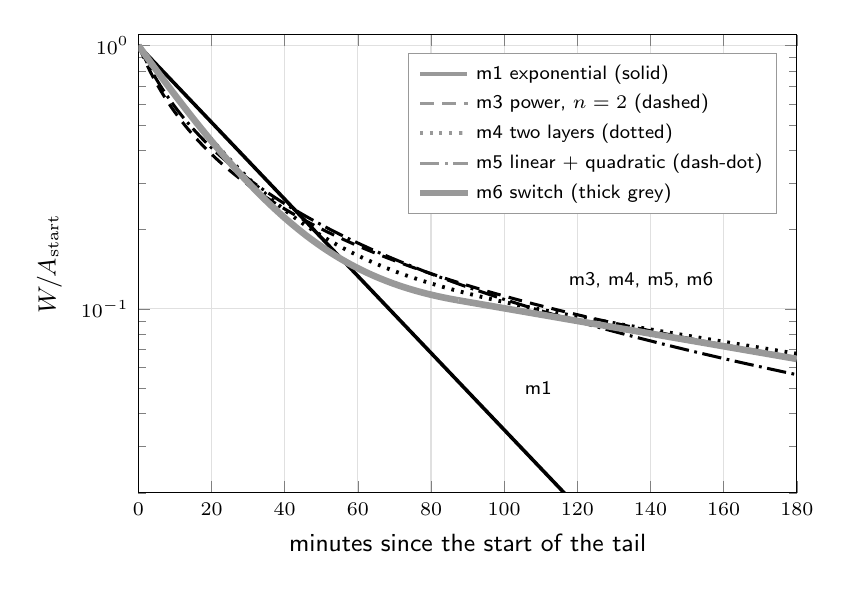
\begin{tikzpicture}
\begin{axis}[width=0.82\linewidth, height=7.4cm, xmin=0, xmax=180, ymin=0.02, ymax=1.1, ymode=log,
  xlabel={minutes since the start of the tail}, ylabel={$W / \Astart$},
  tick label style={font=\sffamily\scriptsize}, label style={font=\sffamily\small},
  legend style={font=\sffamily\scriptsize, draw=black!40, fill=white, at={(0.97,0.96)}, anchor=north east}, legend cell align=left,
  grid=major, grid style={black!12}]
\addplot[domain=0:180, samples=2, line width=1.3pt] {exp(-x/29.75)};
\addlegendentry{m1 exponential (solid)}
\addplot[domain=0:180, samples=60, smooth, line width=1.1pt, dash pattern=on 5pt off 3pt] {1/(1+0.07944*x)};
\addlegendentry{m3 power, $n=2$ (dashed)}
\addplot[domain=0:180, samples=60, smooth, line width=1.4pt, dash pattern=on 1pt off 2.5pt] {0.8286*exp(-x/18.73)+0.1714*exp(-x/193)};
\addlegendentry{m4 two layers (dotted)}
\addplot[domain=0:180, samples=60, smooth, line width=1.1pt, dash pattern=on 7pt off 2pt on 1pt off 2pt] {0.00299*exp(-0.00299*x)/(0.00299+0.067485*(1-exp(-0.00299*x)))};
\addlegendentry{m5 linear + quadratic (dash-dot)}
\addplot[domain=0:87.5, samples=50, smooth, line width=2.4pt, black!40] {(0.1433+1.3567*exp(-0.04928*x))/1.5};
\addlegendentry{m6 switch (thick grey)}
\addplot[domain=87.5:180, samples=2, line width=2.4pt, black!40, forget plot] {0.16148*exp(-0.00554*(x-87.5))/1.5};
\node[font=\sffamily\scriptsize, anchor=west] at (axis cs:103,0.05) {m1};
\node[font=\sffamily\scriptsize, anchor=south west] at (axis cs:115,0.11) {m3, m4, m5, m6};
\end{axis}
\end{tikzpicture}
\caption{The five laws with the parameters calibrated to the real median tail, for a tail that starts at $1.5\dB$,
before any tail-to-tail spread or noise is added. On this logarithmic scale the exponential is a straight line; the
others bend, and they lie almost on top of each other, which is why they are hard to tell apart. The laws were
calibrated together with a spread (Section~\ref{sec:sim}), so a single curve is not expected to match the real median
by itself.}
\label{fig:laws}
\end{figure}

\subsection{The simulator}
\label{sec:sim}

\subsubsection*{Tail-to-tail spread}

Real tails do not all dry at the same speed: antennas differ, and so do wind, sun and temperature. The simulator
gives each tail its own speed by stretching time,
\begin{equation}
W_{i}(t) = W\!\left(\frac{t}{f_{i}}\right), \qquad f_{i} = e^{\,s\,z_{i}}, \qquad
z_{i} = \tfrac{1}{\sqrt{2}}\,z_{\text{link}} + \tfrac{1}{\sqrt{2}}\,z_{\text{tail}}, \quad z \sim \mathcal{N}(0,1),
\label{eq:spread}
\end{equation}
so half of the variation belongs to the link (it is the same in all its tails) and half to the single tail. The
width $s$ is set so that the band between the 10th and 90th percentile of the simulated tails matches the real band;
this gives $s = 1.25$ for every law, i.e.\ individual tails dry between 5 times faster and 5 times slower than the
median.

\subsubsection*{The measurement chain}

A real tail is not $W(t)$; it is $W(t)$ seen through the instrument. The simulator applies the same chain
(Figure~\ref{fig:obs}):
\begin{equation}
x(t) = W_{i}(t) + c_{i} + n_{\mathrm{slow}}(t) + \sigma_{w}\,\varepsilon(t), \qquad
A(t) = \text{1-minute mean of } \; Q_{0.3\dB}\bigl[x(t)\bigr],
\label{eq:obs}
\end{equation}
with $c_{i} \sim \mathcal{N}(0,\sigma_{\mathrm{off}}^{2})$ a constant baseline error of that tail (from the baseline
validation), $n_{\mathrm{slow}}$ a slowly wandering noise, $\varepsilon$ white noise on the 10-second samples, and
$Q$ the rounding of RSL to steps of $0.3\dB$.

\begin{figure}[H]
\centering
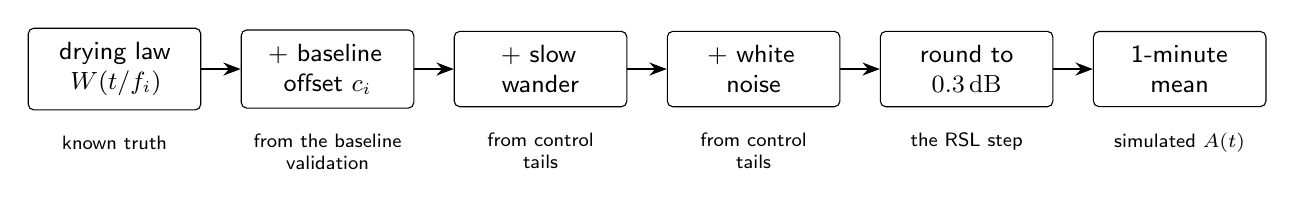
\begin{tikzpicture}[node distance=5mm]
\node[box, text width=18.4mm] (law) {drying law\\$W(t/f_{i})$};
\node[box, text width=18.4mm, right=of law] (off) {+ baseline\\offset $c_{i}$};
\node[box, text width=18.4mm, right=of off] (slow) {+ slow\\wander};
\node[box, text width=18.4mm, right=of slow] (white) {+ white\\noise};
\node[box, text width=18.4mm, right=of white] (q) {round to\\$0.3\dB$};
\node[box, text width=18.4mm, right=of q] (m) {1-minute\\mean};
\draw[arr] (law)--(off); \draw[arr] (off)--(slow); \draw[arr] (slow)--(white); \draw[arr] (white)--(q); \draw[arr] (q)--(m);
\node[lab, below=2mm of law] {known truth};
\node[lab, below=2mm of off] {from the baseline\\validation};
\node[lab, below=2mm of slow] {from control\\tails};
\node[lab, below=2mm of white] {from control\\tails};
\node[lab, below=2mm of q] {the RSL step};
\node[lab, below=2mm of m] {simulated $A(t)$};
\end{tikzpicture}
\caption{The simulator: a known law seen through the measurement chain. Each block can be switched off to see which
distortion hides what.}
\label{fig:obs}
\end{figure}

\subsubsection*{Getting the noise right}

The first version of the simulator had only white noise. Compared with the real control tails (which contain noise
and no drying), it was far too quiet over a whole tail: the spread within a tail was $0.05\dB$ simulated against
$0.14\dB$ real. Real dry-weather noise is correlated in time: it wanders. A simulator without that would have made
the laws look much easier to tell apart than they are. The noise model was therefore extended with a slow component
(a first-order autoregressive process with its own strength and correlation time), fitted per sub-link to five
properties of its control tails. After the change all five agree (Table~\ref{tab:noise}).

\begin{table}[H]
\centering
\caption{Real dry-weather noise against the simulated noise (medians over sub-links). The typical fitted noise is a
white part of $0.09\dB$, a slow part of $0.15\dB$ and a correlation time of 80 minutes.}
\label{tab:noise}
\small
\begin{tabular}{@{}lcc@{}}
\toprule
Property of a control tail & Real & Simulated \\
\midrule
Spread within the tail (dB) & 0.141 & 0.134 \\
Share of minutes exactly on a $0.3\dB$ level & 0.25 & 0.27 \\
Correlation between minutes 1 minute apart & 0.80 & 0.80 \\
Correlation between minutes 10 minutes apart & 0.57 & 0.63 \\
Correlation between minutes 60 minutes apart & 0.22 & 0.23 \\
\bottomrule
\end{tabular}
\end{table}

\subsubsection*{Calibrating the laws, and a second lesson}

Each law's parameters were set so that its simulated median tail matches the real one
(Table~\ref{tab:calib}, Figure~\ref{fig:realsim}).

\begin{table}[H]
\centering
\caption{Calibrated laws (times in minutes) and how far the simulated median and band are from the real ones (root
mean square difference of $A/\Astart$ over the first 6 hours, after the full measurement chain).}
\label{tab:calib}
\small
\begin{tabular}{@{}llcc@{}}
\toprule
Law & Calibrated parameters & Misfit of the median & Misfit of the band \\
\midrule
m1 exponential & $\tau = 29.8$ & 0.026 & 0.062 \\
m3 power & $c = 0.053$, $n = 2$ & 0.044 & 0.072 \\
m4 two layers & $\tau_{f} = 18.7$, $\tau_{s} = 193$, $\varphi = 0.17$ & 0.033 & 0.062 \\
m5 linear + quadratic & $a = 0.0030$, $b = 0.045$ & 0.038 & 0.069 \\
\bottomrule
\end{tabular}
\end{table}

\begin{figure}[p]
\centering
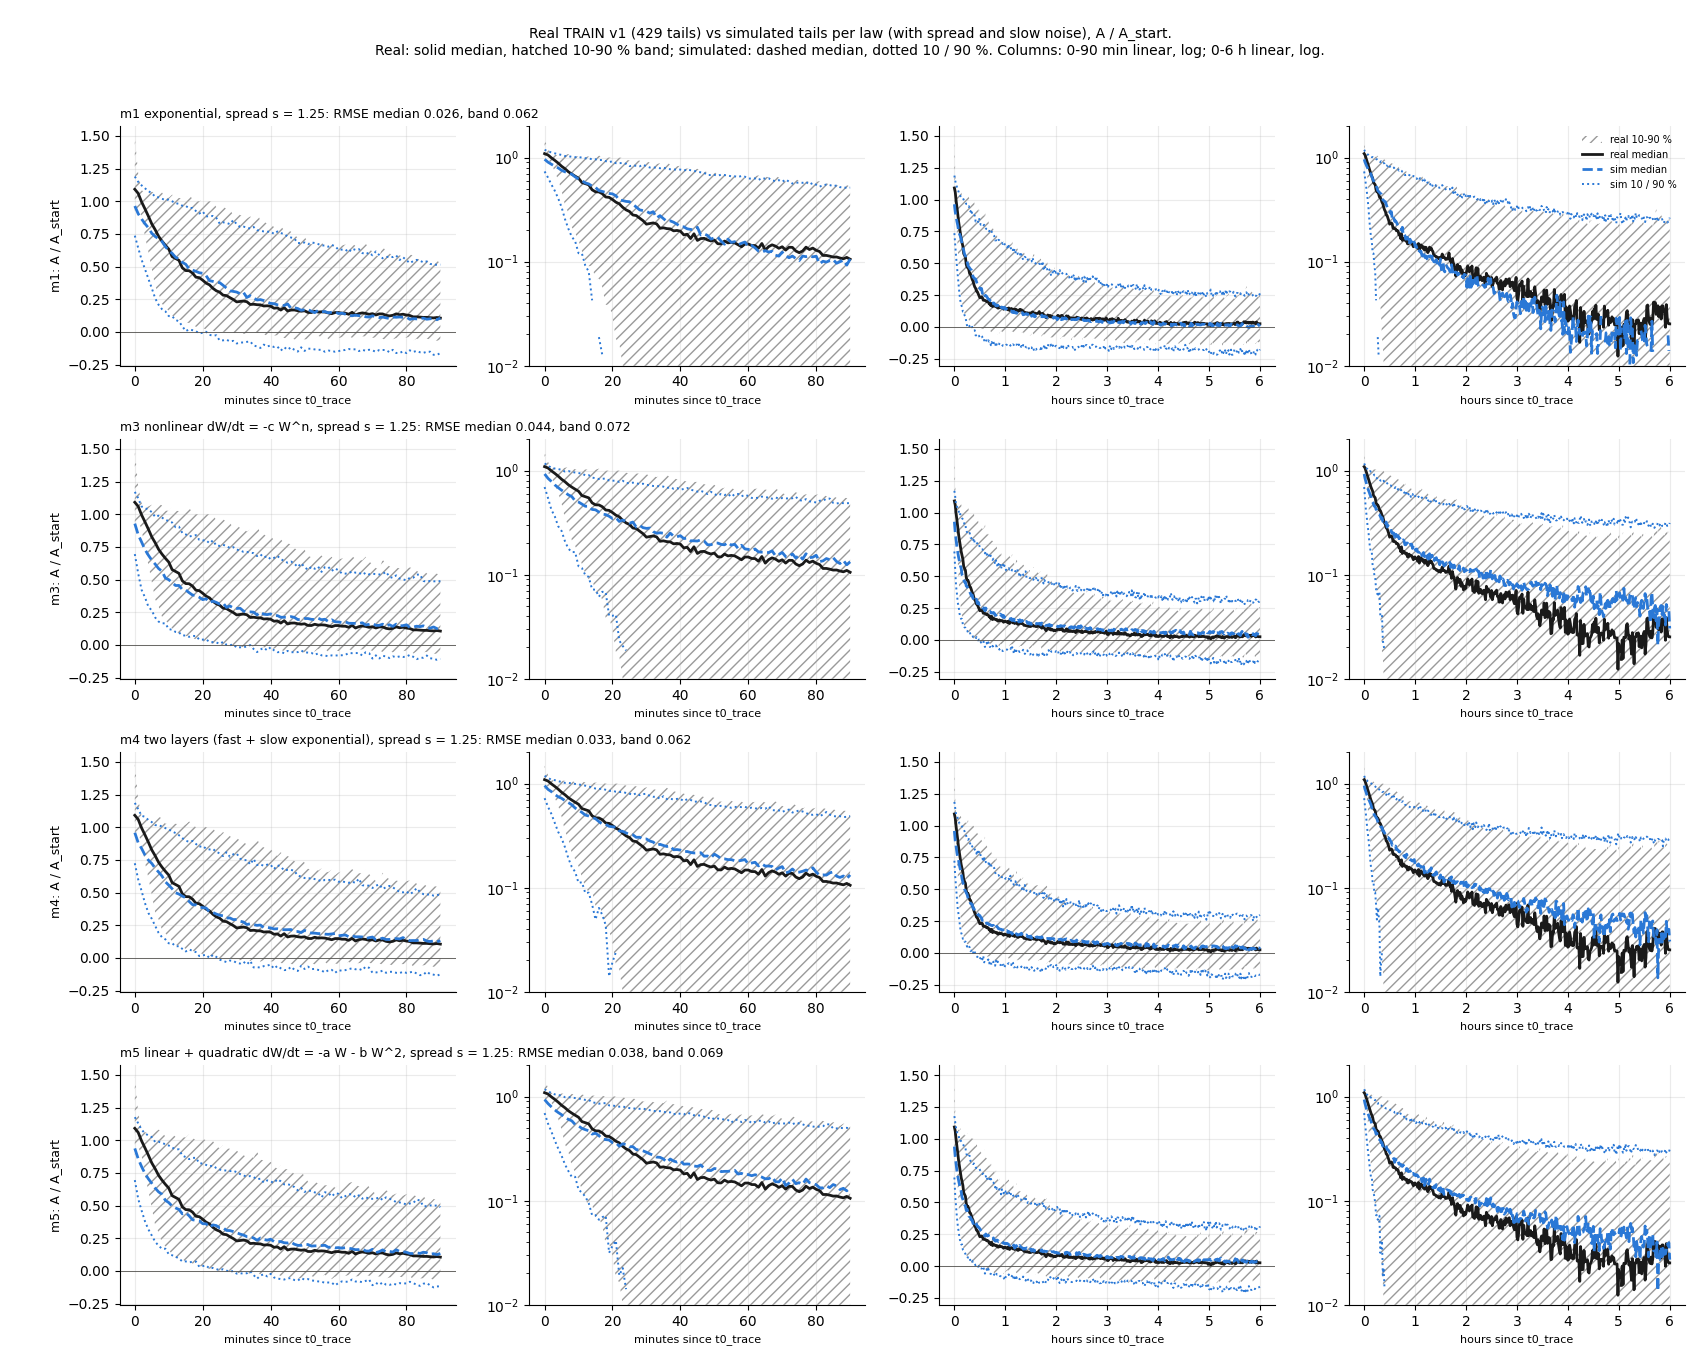
\includegraphics[width=\linewidth]{../research/WAA_estm/outputs/figures/step3a_real_vs_sim_median.png}
\caption{Real tails against simulated tails, one row per law (m1, m3, m4, m5). Solid line and hatched band: real
median and 10--90\,\% band. Dashed and dotted lines: the same for the simulated tails. Columns: first 90 minutes
(linear, logarithmic), first 6 hours (linear, logarithmic). All four laws reproduce the real median and band about
equally well.}
\label{fig:realsim}
\end{figure}

The important result is in the first row of the table. Before the spread was added, the plain exponential could not
produce the slow remainder of the real median, and two layers fitted best; it looked as if the data asked for two
layers. With the spread, the noise, the offsets and the real tail lengths included, \textbf{a plain exponential
reproduces the slow remainder as well as two layers do}. A population of antennas that each dry exponentially but at
different speeds looks, in the median, like one antenna with a fast and a slow layer. The shape of the median curve
therefore cannot decide between the laws; the decision has to come from the individual tails.

\subsection{Fitting one tail at a time: not enough}
\label{sec:pertail}

The natural first method fits every candidate to every tail separately, each with its own start and its own constant
offset, and picks the candidate with the best score. The score is the Bayesian information criterion (BIC), which
rewards a good fit and charges for every extra parameter. Because the noise wanders, neighbouring minutes are not
independent, and a tail of $n$ minutes carries less information than $n$ independent values. This is accounted for by
an effective sample size:
\begin{equation}
n_{\mathrm{eff}} = n\,\frac{1-\rho}{1+\rho}, \qquad
\mathrm{BIC} = n_{\mathrm{eff}}\,\ln\!\frac{\mathrm{RSS}}{n} + k\,\ln n_{\mathrm{eff}},
\end{equation}
where $\rho$ is the correlation between neighbouring residuals, RSS the sum of squared residuals and $k$ the number of
parameters. A typical tail has $n = 210$ minutes but only $n_{\mathrm{eff}} \approx 64$.

Applied to simulated data sets with each of the five laws as the truth (ten data sets per law), the result was
negative, and clearly so:
\begin{itemize}
\item \textbf{Per tail, nothing can be identified.} The exponential wins 60 to 80\,\% of the tails whatever the true
law is. One noisy, quantized tail that starts near $1.5\dB$ does not contain enough information.
\item \textbf{Per data set} (scores summed over all tails), only one question can be answered: \emph{single
exponential or not}. When the truth is exponential, the exponential wins every time. When the truth is any of the
other four laws, the two-layer candidate wins. So if two layers won on real data, it would mean ``not a single
exponential'', and not ``two layers''.
\item The slow time constant of the two-layer law cannot be recovered: the fit trades it against the free offset.
\item Switching the distortions off one at a time showed that no single one is to blame. Noise alone, or quantization
alone, is enough to hide the small slow layer.
\end{itemize}

\subsection{Fitting all tails together: works on simulated data}
\label{sec:pooled}

The weakness of the per-tail fit is that every tail gets its own free parameters and no tail informs another. But the
question is not ``what is the law of this tail''; it is ``what is the one law that all antennas follow''. The second
method asks exactly that. One candidate law with one set of parameters $\theta$ is fitted to the whole data set at
once:
\begin{equation}
A_{i}(t) \;=\; W\!\left(\frac{t}{f_{i}};\ \theta,\ W_{0,i}\right) + c_{i} + e_{i}(t) .
\label{eq:pooled}
\end{equation}
The pieces, and what each one fixes compared with the per-tail fit:
\begin{itemize}
\item $\theta$: the law's parameters, \textbf{shared by all tails}. This is where the information is pooled.
\item $W_{0,i}$: the start of tail $i$, free.
\item $f_{i} = e^{\,s(u_{\text{link}} + v_{\text{tail}})}$: the speed of tail $i$, as in Eq.~\eqref{eq:spread}. It is
not fitted per tail. It is treated as a random quantity with a width $s$ that is fitted, and the likelihood is
\emph{averaged} over all the speeds a tail could have. This is what separates ``many exponentials with different
speeds'' from ``two layers''.
\item $c_{i}$: the offset of tail $i$, no longer free. It has the prior
$c_{i} \sim \mathcal{N}(0, \sigma_{\mathrm{off}}^{2})$, with $\sigma_{\mathrm{off}}$ the baseline error of that
sub-link measured in dry weather. The offset can no longer absorb a slow layer for free.
\item $e_{i}(t)$: the noise, with the white and the slow part of that sub-link measured on its control tails. The
likelihood uses this correlated-noise model directly, instead of correcting for it afterwards.
\end{itemize}
Schematically, the quantity that is maximised over $\theta$ and $s$ is
\begin{equation}
\mathcal{L}(\theta, s) \;=\; \prod_{\text{links}} \int\! du\; p(u) \prod_{i \,\in\, \text{link}} \int\! dv\; p(v)\;
\max_{W_{0,i},\,c_{i}}\; p\bigl(A_{i} \,\big|\, \theta, W_{0,i}, c_{i}, f_{i}\bigr)\,p(c_{i}),
\end{equation}
and the candidates are compared by $\mathrm{BIC} = -2\ln\mathcal{L} + k\ln N$, where $N$ counts the independent units (a link in an event), not the minutes and not the tails.

\subsubsection*{The test and its result}

The test data follow the structure of the real set. Ten data sets per true law were built by an \emph{event
bootstrap}: 24 events are drawn with replacement from the 24 real ones, with all their tails, so that the dominance of
a few events is part of the test. A rule for success was written down before the run: the method is useful if the
true law's own candidate wins in at least 80\,\% of the data sets for the exponential, two-layer, linear + quadratic
and switch laws, and the main parameters are recovered within $\pm 30\,\%$.

The rule was met, using the first 60 minutes of each tail, the first 6 hours, or the whole tail
(Figure~\ref{fig:confusion}):
\begin{itemize}
\item The right law wins in 80 to 100\,\% of the data sets for the four laws in the rule.
\item The parameters come back within about $\pm 15\,\%$ (median), including the slow time constant and the share of
the slow layer, which the per-tail fit could not recover.
\item One confusion remains: the pure power law (m3) is taken for the linear + quadratic law (F5) in 20 to 40\,\% of
its data sets. The two are close relatives, and F5 contains a quadratic term.
\end{itemize}

\begin{figure}[H]
\centering
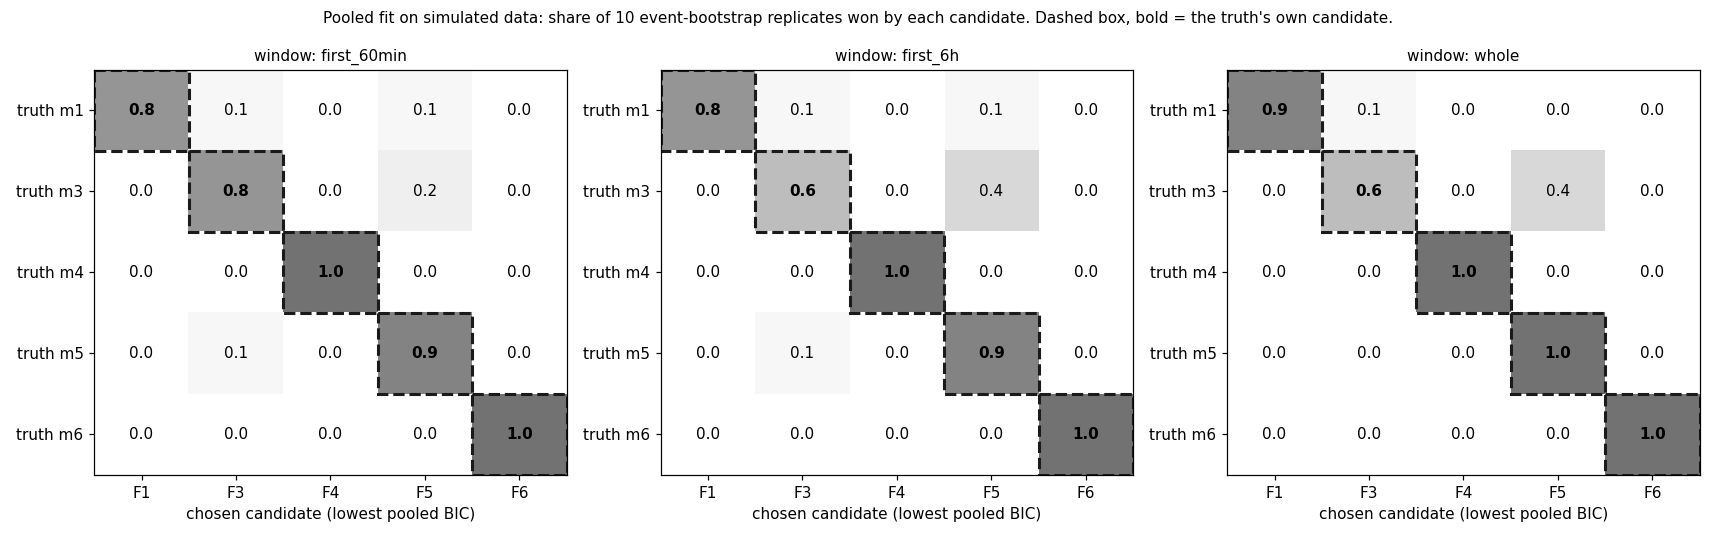
\includegraphics[width=\linewidth]{../research/WAA_estm/outputs/figures/step3b1b_confusion.png}
\caption{Pooled fit on simulated data. Rows: the law that generated the data. Columns: the candidate chosen. Each cell
is the share of the ten data sets; a perfect method would have 1.0 on the diagonal (dashed boxes). Panels: first 60
minutes, first 6 hours, whole tail.}
\label{fig:confusion}
\end{figure}

\subsubsection*{What this does and does not show}

On the real tails, the pooled fit will be able to say which of the five forms describes the drying best, with its
parameters and an uncertainty from resampling events. It will not prove a mechanism: the true law may be none of the
five, and the winner is then only the best approximation among them. And the test above was run under friendly
conditions, which is why the next step was added:
\begin{itemize}
\item the fit used the same noise model that generated the data, while the real noise has more than one time scale;
\item the search started from the calibrated parameters of each law;
\item the real tails decay faster in the first hour than every calibrated law (real median $A/\Astart$ at 30 minutes
is $0.23$; the simulated laws give $0.28$ or more). This is a hint, not a result: the uncertainty of the real value
is wide ($0.16$ to $0.56$).
\end{itemize}

\subsection{Stress test of the pooled fit: partly passed}
\label{sec:stress}

The stress test tries to break the pooled fit by removing the three friendly conditions one at a time, again on
simulated data and again with a rule for success fixed before the run (per test and per true law: the law's own
candidate wins in at least 4 of 5 data sets, and its main parameters come back within $\pm 30\,\%$). It uses the first
60 minutes of each tail and four true laws: exponential, two layers, linear + quadratic, and the switch.
\begin{description}[leftmargin=1.2cm, style=nextline]
\item[T1, wrong noise model.] The data are generated with two slow noise components (correlation times of 20 and 300
minutes), but the fit still assumes one. Slow noise that the fit does not model could be mistaken for a slow layer and
favour the more flexible laws.
\item[T2, honest starting points.] The search starts from four generic values, the same for every true law, instead
of from the right answer; the best of the four is kept.
\item[T3, faster truths.] Every law is recalibrated to the real median at 10, 30 and 60 minutes, so that the test
data dry as fast as the real tails do. The exponential and the two-layer law are also tested with a wider spread of
drying speeds ($s = 1.5$).
\end{description}

\begin{table}[H]
\centering
\caption{Stress test of the pooled fit on simulated data: 12 of the 14 cases pass. ``Pass'' means the rule fixed before
the run is met.}
\label{tab:stress}
\small
\begin{tabularx}{\linewidth}{@{}l c c Y@{}}
\toprule
True law & T1: wrong noise & T2: honest starts & T3: faster truths \\
\midrule
m1 exponential & pass & pass & pass (also with the wider spread) \\
m4 two layers & pass & pass & pass (also with the wider spread) \\
m6 switch & pass & pass & pass \\
m5 linear + quadratic & \textbf{fail}: the power law wins 5 of 5 & pass & \textbf{fail}: wins 4 of 5, but its linear rate comes back at 0.65 of the truth \\
\bottomrule
\end{tabularx}
\end{table}

What the result means:
\begin{itemize}
\item \textbf{The method holds for three of the four laws.} The exponential, the two-layer law and the switch are
recognised under noise the fit does not know, from generic starting points, and when they dry as fast as the real
tails. The fear that unmodelled slow noise would be mistaken for a slow layer did not come true in this test.
\item \textbf{The two nonlinear laws are one family.} Both failures belong to the linear + quadratic law, and both
have the same cause: with the calibrated parameters its linear term is small, so it is almost a pure quadratic, which
the power law copies. The margins are tiny (about 2 BIC units, in either direction). On real tails the two will be
read together as ``drying that speeds up when the antenna is wetter'', and the linear rate will not be interpreted
from the first hour.
\item \textbf{Starting points matter, most of all for the switch law.} From different starting points the switch
candidate reached clearly different solutions in all 20 data sets of the test, the other candidates in about a fifth to
a half of them. The winner still was the same as with the ideal start in 19 of 20 data sets. Every candidate will
therefore be fitted from several starting points on the real tails.
\item \textbf{Two layers against the switch needs a clear margin.} In one two-layer data set the switch won from a
generic start by about 4 BIC units; a difference below about 10 units between these two will not be called a
decision.
\end{itemize}
One limit of the test itself: when the slow laws were recalibrated to the fast early decay with all parameters free,
their slow part ran off to a constant floor, so the slow parameters were kept at their earlier values. This choice was
made before any fit of T3 and is still to be confirmed by us.

\inshort{A simulator that copies the real tails and their noise shows that the median curve cannot decide between the
laws, and that fitting single tails cannot either. Fitting all tails together, with a shared law, a random speed per
tail, a bounded offset and a correlated-noise model, recovers the right law and its parameters on simulated data. A
stress test confirms this for the exponential, the two-layer and the switch law; the two nonlinear laws cannot be
separated from each other. All of this is on simulated data: no law has been fitted to the real tails.}

% =====================================================================================================================
\section{Where we stand}
\label{sec:stand}

\begin{table}[H]
\centering
\caption{What is established, and what is not, on 11 October 2026.}
\label{tab:stand}
\small
\begin{tabularx}{\linewidth}{@{}Y Y@{}}
\toprule
\textbf{Established} & \textbf{Not established yet} \\
\midrule
$A(t)$ exists for every training and validation event on the training links, with a baseline that is unbiased and accurate to about one quantization step. &
Baselines for the test events and test links (needed for the final held-out check). \\
The baseline does not absorb the drying after rain. &
Whether the attenuation at the start of a tail is the antenna or residual light rain on the path. \\
A memory after rain exists: strong tails take hours to return to the dry level. &
The form of the drying law. No law has been fitted to real tails. \\
A frozen, non-circular set of 429 drying tails (and 123 validation tails not yet looked at). &
What the unexplained night-time rises are (drizzle or condensation). \\
The median tail halves in about 15 minutes and has a slow remainder. &
Whether the slow remainder is a second process or only the spread of drying speeds between antennas. \\
The median curve and single-tail fits cannot identify the law; a pooled fit can, on simulated data, also under a wrong noise model and from generic starting points (exponential, two layers, switch). &
Whether SINDy recovers a known law from simulated tails (not tested yet). \\
On simulated data the power law and the linear + quadratic law cannot be told apart. &
Which law the real tails follow, and whether the real noise is close enough to the two noise models tested. \\
Dry-weather noise is correlated over tens of minutes; dew produces WAA-like jumps at night. &
The wetting law, the path law $f$, and the rain estimate: not started. \\
\bottomrule
\end{tabularx}
\end{table}

Two methodological habits have carried the work so far and will continue. The first is to \emph{build a case with a
known truth} before trusting a method: fake events for the baseline, simulated tails for the fitting. The second is to
\emph{fix the decision rule before the run}: the rejected humidity rule, the tail selection, and the success rules of
the fitting tests were all written down before their results were seen. Twice this prevented a wrong conclusion that
looked attractive: that the fast drop is antenna drying (Section~\ref{sec:fastdrop}) and that the data ask for two
layers (Section~\ref{sec:sim}). The stress
test adds a third case of the same kind: a win of the linear + quadratic law over the power law, or the reverse, will
not be read as a finding.

% =====================================================================================================================
\section{What comes next}
\label{sec:next}

\subsection{The target of Stage 1}

The goal is one dynamic equation for the WAA with rain as its input,
\begin{equation}
\frac{dW}{dt} \;=\; \underbrace{g(R, W)}_{\text{wetting}} \;-\; \underbrace{h(W)}_{\text{drying}} ,
\label{eq:target}
\end{equation}
where $h$ is learned from the drying tails ($R = 0$, so $dW/dt = -h(W)$) and $g$ from whole events on very short
links, where the path term is small. Figure~\ref{fig:plan} shows the route.

\begin{figure}[H]
\centering
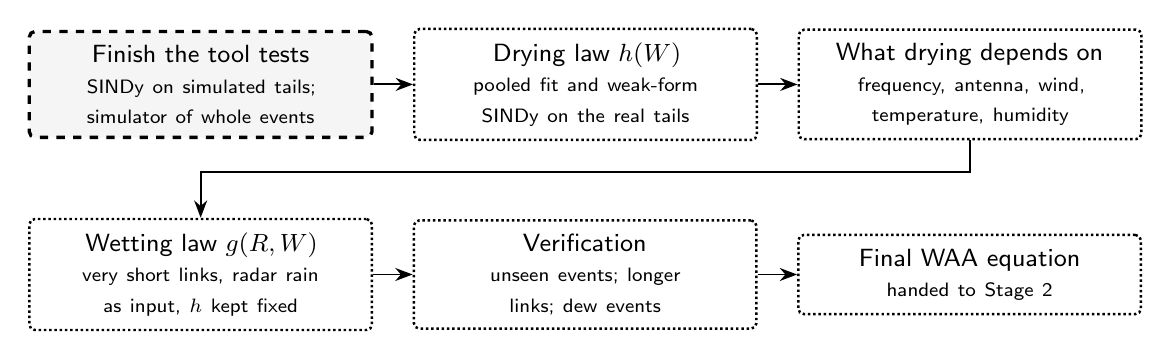
\begin{tikzpicture}[node distance=5mm and 5mm]
\node[doing, text width=40mm] (a) {Finish the tool tests\\{\scriptsize SINDy on simulated tails; simulator of whole events}};
\node[todo, text width=40mm, right=of a] (b) {Drying law $h(W)$\\{\scriptsize pooled fit and weak-form SINDy on the real tails}};
\node[todo, text width=40mm, right=of b] (c) {What drying depends on\\{\scriptsize frequency, antenna, wind, temperature, humidity}};
\node[todo, text width=40mm, below=10mm of a] (d) {Wetting law $g(R,W)$\\{\scriptsize very short links, radar rain as input, $h$ kept fixed}};
\node[todo, text width=40mm, right=of d] (e) {Verification\\{\scriptsize unseen events; longer links; dew events}};
\node[todo, text width=40mm, right=of e] (f) {Final WAA equation\\{\scriptsize handed to Stage 2}};
\draw[arr] (a)--(b); \draw[arr] (b)--(c);
\draw[arr] (c.south) -- ++(0,-4mm) -| (d.north);
\draw[arr] (d)--(e); \draw[arr] (e)--(f);
\end{tikzpicture}
\caption{The remaining route of Stage 1. Dashed border: in progress. Dotted border: planned.}
\label{fig:plan}
\end{figure}

\subsection{The steps}

\begin{enumerate}
\item \textbf{Finish testing the tools.} The stress test is done (Section~\ref{sec:stress}). Next, test weak-form
SINDy [10] on simulated tails: with a library of terms $1, W, W^{2}, W^{3}$ and switch terms $\max(W - A_{c}, 0)$,
does it return the law that generated the data? What does it return when the truth has a hidden second state (two
layers)? Does mixing tails of different speeds create a false nonlinear term? The weak form is used because it
integrates the data against smooth test functions instead of differentiating it, and differentiating a signal
quantized to $0.3\dB$ is hopeless. Last, extend the simulator from tails to whole events (real radar rain, a wetting
law, a small path term that grows with $L$) so that SINDy with rain as input can be tested as well.
\item \textbf{The drying law on real tails.} Fit the five candidates with the pooled method, each from several
starting points, and run SINDy, on the frozen set. Every result is repeated on four versions of the set (the main set; without the flagged events; without
the tails with a level flag; the alternative set), and its uncertainty comes from resampling events. The exponential
drying of the literature is one of the candidates, so the comparison with the literature is built in.
\item \textbf{What drying depends on.} Relate the drying speed to frequency, antenna size, time of day, temperature,
wind and humidity.
\item \textbf{The wetting law, from very short links.} On links shorter than about $0.6$ km the path term is small, so
$A(t)$ during the rain is mostly WAA. That the path term is small must be shown without assuming the power law:
among short links, the attenuation during rain must not grow with $L$, and the two directions of a link must agree.
With $h(W)$ kept fixed from the tails, $g(R,W)$ is learned with SINDy using the radar rain along the path as input,
and compared with the model of Schleiss et al.\ [1]. This step is also the real test of whether what we call WAA
belongs to the antenna (Section~\ref{sec:fastdrop}).
\item \textbf{Verification.} On data not used so far: drying on the validation events; the full law on unseen events;
agreement between the drying time found by SINDy and the one fitted directly; agreement between the two directions of
a link; and whether dew events, which wet the antenna without rain, dry by the same $h(W)$. The decisive check is the
transfer to longer links: after the predicted WAA is subtracted, the remaining attenuation should grow with $L$ with
no constant offset. That is the test of Eq.~\eqref{eq:L0}, and it is the handover to Stage~2.
\end{enumerate}

\subsection{After Stage 1}

\begin{itemize}
\item \textbf{Stage 2, the path law.} With the WAA removed, learn $f(L,\Rbar,Z)$ of Eq.~\eqref{eq:f} by symbolic
regression (PySR [7]), with the radar rain along the path as the reference, and see how the dependence on the length
differs from $f = L$.
\item \textbf{Rain estimate and evaluation.} Invert the combined model (path law and WAA) to get rain from
attenuation, on events that were not used for training. Measures: normalised bias and normalised RMSE against gauges
and radar, by link length; the amount of false rain after the end of events; comparison with the plain power law, the
WAA models of the literature [1], [9] and a neural-network reference [11]; and the stability of the learned terms
under resampling.
\end{itemize}

\subsection{Open questions}

\begin{itemize}
\item Are the night-time rises after rain drizzle that the radar misses, or condensation? The humidity record has
gaps exactly there.
\item Should light rain after the first dry moment end a tail (as now), or be given to the model as input?
\item The spread of drying speeds was calibrated after the noise was fixed, so any noise the model still misses ends
up in the spread. How much of $s = 1.25$ is real variation between antennas?
\item The literature form for exponential drying is named in the working plan after Minda and Nakamura; that
reference is not in the proposal's list and has to be checked and added before it is cited.
\end{itemize}

% =====================================================================================================================
\section*{References}
\addcontentsline{toc}{section}{References}

The numbers are those of the project proposal; only the references used in this report are listed.

\begin{description}[leftmargin=1.1cm, labelwidth=0.9cm, labelsep=0.2cm, font=\normalfont]
\item[{[1]}] Schleiss, M., Rieckermann, J., \& Berne, A. (2013). Quantification and modeling of wet-antenna
attenuation for commercial microwave links. \emph{IEEE Geoscience and Remote Sensing Letters}, 10(5), 1195--1199.
\item[{[7]}] Cranmer, M. (2023). Interpretable machine learning for science with PySR and SymbolicRegression.jl.
arXiv:2305.01582.
\item[{[8]}] Ostrometzky, J., \& Messer, H. (2018). Dynamic determination of the baseline level in microwave links
for rain monitoring from minimum attenuation values. \emph{IEEE Journal of Selected Topics in Applied Earth
Observations and Remote Sensing}.
\item[{[9]}] Pastorek, J., Fencl, M., Rieckermann, J., \& Bare\v{s}, V. (2021). Precipitation estimates from
commercial microwave links: practical approaches to wet-antenna correction. \emph{IEEE Transactions on Geoscience and
Remote Sensing}.
\item[{[10]}] Messenger, D. A., \& Bortz, D. M. (2021). Weak SINDy: Galerkin-based data-driven model selection.
\emph{Multiscale Modeling \& Simulation}, 19(3), 1474--1497.
\item[{[11]}] Habi, H. V., \& Messer, H. (2020). Recurrent neural network for rain estimation using commercial
microwave links. \emph{IEEE Transactions on Geoscience and Remote Sensing}.
\item[{[13]}] Andersson, J. C. M., Olsson, J., van de Beek, R., \& Hansryd, J. (2022). OpenMRG: open data from
microwave links, radar, and gauges for rainfall quantification in Gothenburg, Sweden. \emph{Earth System Science
Data}, 14, 5411--5426.
\end{description}

% =====================================================================================================================
\appendix
\section{Glossary}

\begin{tabularx}{\linewidth}{@{}l Y@{}}
\toprule
\textbf{Term} & \textbf{Meaning} \\
\midrule
$A(t)$ & Attenuation: total loss minus baseline, Eq.~\eqref{eq:A}. \\
$\Arain$, $\delta(t)$ & The part of $A$ caused by rain along the path; everything else. \\
$W(t)$ & Wet-antenna attenuation (WAA), in dB. \\
$\Rbar$, $L$ & Mean rain rate along the path; path length. \\
$f(L,\Rbar,Z)$ & The path-law correction to be learned in Stage 2; uniform rain gives $f = L$. \\
Sub-link & One direction of a two-way link. \\
Baseline & The total loss of a sub-link without rain; here one number per (event, sub-link). \\
Fake event & A pretended event placed in certified dry weather, where the true attenuation is zero. \\
Offset, $\sigma_{\mathrm{off}}$ & The baseline error of one (fake) event; its spread for a sub-link. \\
Drying tail & The stretch of $A(t)$ after the rain has stopped on a link. \\
$\tzero$, $\ttrace$ & End of the link's last wet bin; end of the last bin with any trace of rain (the tail start). \\
$\Astart$ & Mean of $A$ over the first 5 minutes of the tail. \\
Control tails & Tails that start below $0.5\dB$: noise without drying. \\
Tail set v1 & The frozen set of 429 training tails (123 validation). \\
m1 \ldots m6, F1 \ldots F6 & A drying law used as the truth of a simulation; the same law used as a candidate in a fit. \\
Spread $s$ & Width of the tail-to-tail variation of the drying speed, Eq.~\eqref{eq:spread}. \\
BIC & Bayesian information criterion: goodness of fit with a charge per parameter; lower is better. \\
Pooled fit & One law with shared parameters fitted to all tails at once, Eq.~\eqref{eq:pooled}. \\
Event bootstrap & Resampling whole events with replacement, to measure uncertainty. \\
SINDy & Sparse identification of nonlinear dynamics: finds a short equation for $dW/dt$ from a library of terms. \\
\bottomrule
\end{tabularx}

\section{Where the details are}
\label{app:where}

This report gives the ideas. The exact rules, thresholds and numbers are in the documents of each module, inside the
research folder.

{\small
\begin{tabularx}{\linewidth}{@{}l Y@{}}
\toprule
\textbf{Topic} & \textbf{Document} \\
\midrule
Baseline method, flags, accuracy & \code{baseline\_estm/METHOD.md} \\
Baseline validation & \code{R1\_validation.md} and \code{R1b\_validation.md}, in the reports folder of \code{baseline\_estm} \\
Tail definitions, rules of set v1 & \code{WAA\_estm/README.md} \\
What each WAA step decided & \code{WAA\_estm/DECISIONS.md} \\
Frozen tail set & \code{step2c\_freeze.md}, in the reports folder of \code{WAA\_estm} \\
Simulator and its calibration & \code{step3a\_fix.md}, same folder \\
Pooled fit on simulated tails & \code{step3b1b\_pooled\_fit.md}, same folder \\
The WAA plan & \code{WAA\_estm/roadmap.md} \\
The data layer & \code{docs/pipeline\_log.pdf} (next to this report) \\
\bottomrule
\end{tabularx}}

\end{document}
